%---------------------------------------------------------------------------
% scrlttr2.tex v0.3. (c) by Juergen Fenn <juergen.fenn@gmx.de>
% Template for a letter to be typeset with scrlttr2.cls from KOMA-Script.
% Latest version of the LaTeX Project Public License is applicable. 
% File may not be modified and redistributed under the same name 
% without the author's prior consent.
%---------------------------------------------------------------------------
\documentclass%%
%---------------------------------------------------------------------------
  [fontsize=12pt,%%          Schriftgroesse
%---------------------------------------------------------------------------
% Satzspiegel
   paper=a4,%%               Papierformat
   enlargefirstpage=on,%%    Erste Seite anders
   firstfoot=off,
   pagenumber=right,%%   Seitenzahl oben mittig
%---------------------------------------------------------------------------
% Layout
   headsepline=off,%%         Linie unter der Seitenzahl
   parskip=half,%%           Abstand zwischen Absaetzen
%---------------------------------------------------------------------------
% Briefkopf und Anschrift
   fromalign=right,%%        Plazierung des Briefkopfs
   fromphone=off,%%           Telefonnummer im Absender
   fromrule=off,%%           Linie im Absender (aftername, afteraddress)
   fromfax=off,%%            Faxnummer
   fromemail=on,%%          Emailadresse
   fromurl=off,%%            Homepage
   fromlogo=off,%%           Firmenlogo
   addrfield=on,%%           Adressfeld fuer Fensterkuverts
   backaddress=on,%%          ...und Absender im Fenster
   subject=beforeopening,%%  Plazierung der Betreffzeile
   locfield=narrow,%%        zusaetzliches Feld fuer Absender
   foldmarks=on,%%           Faltmarken setzen
   numericaldate=off,%%      Datum numerisch ausgeben
   refline=narrow,%%         Geschaeftszeile im Satzspiegel
%---------------------------------------------------------------------------
% Formatierung
   draft=off,%%                Entwurfsmodus
   %backaddress=plain%%        Keine Linie unter Absender
  DIV=12
]{scrlttr2}
%---------------------------------------------------------------------------
\usepackage[english,ngerman]{babel}
\usepackage[T1]{fontenc}
\usepackage[utf8]{inputenc}
\usepackage{url}
\usepackage{lmodern}
\usepackage{csquotes}
\usepackage{pdfpages}
\usepackage{graphics}
%---------------------------------------------------------------------------
% Fonts
\setkomafont{fromname}{\sffamily}
\setkomafont{fromaddress}{\sffamily}%% statt \small
\setkomafont{pagenumber}{\sffamily}
\setkomafont{subject}{\mdseries}
\setkomafont{backaddress}{\mdseries}
\usepackage{mathptmx}%% Schrift Times
%\usepackage{mathpazo}%% Schrift Palatino
%\setkomafont{fromname}{\LARGE}
%---------------------------------------------------------------------------
\usepackage{lastpage}

\renewcommand*{\pagemark}{{\usekomafont{pagenumber}{%
    \pagename\
    \thepage\ von\ \pageref{LastPage}}}}

\begin{document}
%---------------------------------------------------------------------------
% Briefstil und Position des Briefkopfs
\LoadLetterOption{DIN} %% oder: DINmtext, SN, SNleft, KOMAold.
\makeatletter
\@setplength{firstheadvpos}{20mm}
\@setplength{firstheadwidth}{\paperwidth}
\ifdim \useplength{toaddrhpos}>\z@
  \@addtoplength[-2]{firstheadwidth}{\useplength{toaddrhpos}}
\else
  \@addtoplength[2]{firstheadwidth}{\useplength{toaddrhpos}}
\fi
\@setplength{foldmarkhpos}{6.5mm}
\@addtoplength{firstfootvpos}{-10mm}
\makeatother
%---------------------------------------------------------------------------
% Absender
\setkomavar{fromlogo}{\vspace{-1cm}
\includegraphics[width=4cm]{logo.pdf}}
\setkomavar{backaddress}{ZaPF e.V.\\Max-von-Laue-Str. 1\\60438 Frankfurt / Main}
\setkomavar{fromname}{
\includegraphics[width=2cm]{logo.pdf}\\Zusammenkunft aller Physik-Fachschaften\\c/o ZaPF e.V.\\Goethe Universität Frankfurt\\Raum \_\_.208}
\setkomavar{fromaddress}{Max-von-Laue-Str. 1\\60438 Frankfurt / Main}
%\setkomavar{fromphone}{}
%\renewcommand{\phonename}{Telefon}
\setkomavar{fromemail}{stapf@googlegroups.com}
\setkomavar{backaddressseparator}{ – }
\setkomavar{signature}{Björn Guth\\Sprecher des StAPF}
%\setkomavar{frombank}{}
%\setkomavar{location}{\\[8ex]\raggedleft{\footnotesize{\usekomavar{fromaddress}\\
%      Telefon:\ usekomavar{fromphone}}}}%% Neben dem Adressfenster
%---------------------------------------------------------------------------
%\firsthead{Frei gestalteter Briefkopf}
%---------------------------------------------------------------------------
%\firstfoot{}
%---------------------------------------------------------------------------
% Geschaeftszeilenfelder
\setkomavar{place}{Aachen}
\setkomavar{placeseparator}{, den }
\setkomavar{date}{\today}
%\setkomavar{yourmail}{1. 1. 2003}%% 'Ihr Schreiben...'
%\setkomavar{yourref} {abcdefg}%%    'Ihr Zeichen...'
%\setkomavar{myref}{Test}%%      Unser Zeichen
%\setkomavar{invoice}{123}%% Rechnungsnummer
%\setkomavar{phoneseparator}{}
%---------------------------------------------------------------------------
% Versendungsart
%\setlengthtoplength{\fill}{specialmailindent}
%\setkomavar{specialmail}{Einschreiben mit Rückschein}
%---------------------------------------------------------------------------
% Anlage neu definieren
\renewcommand{\enclname}{Anlagen}
\setkomavar{enclseparator}{: }
%---------------------------------------------------------------------------
% Seitenstil
%\pagestyle{plain}%% keine Header in der Kopfzeile
%---------------------------------------------------------------------------
\newcommand{\massmail}[2]{
\begin{letter}{#1}
%---------------------------------------------------------------------------
% Weitere Optionen
\KOMAoptions{%%
}
%---------------------------------------------------------------------------
\setkomavar{subject}{\textbf{Stellungnahme zum Bildungszugang für Geflüchtete}}
%---------------------------------------------------------------------------
\opening{#2}

die Zusammenkunft aller Physikfachschaften hat auf ihrer letzten Tagung am 22.11.2015 die folgende Stellungnahme zum Bildungszugangs für Geflüchtete verabschiedet.

Für Kommentare und Rückfragen stehen wir Ihnen jeder Zeit zur Verfügung und verbleiben 

Mit freundlichen Grüßen,

\closing{Im Auftrag der ZaPF}
%---------------------------------------------------------------------------
%\ps{PS: 134}
%\encl{}
%\cc{Die Menschheit}
%---------------------------------------------------------------------------

%\newpage
%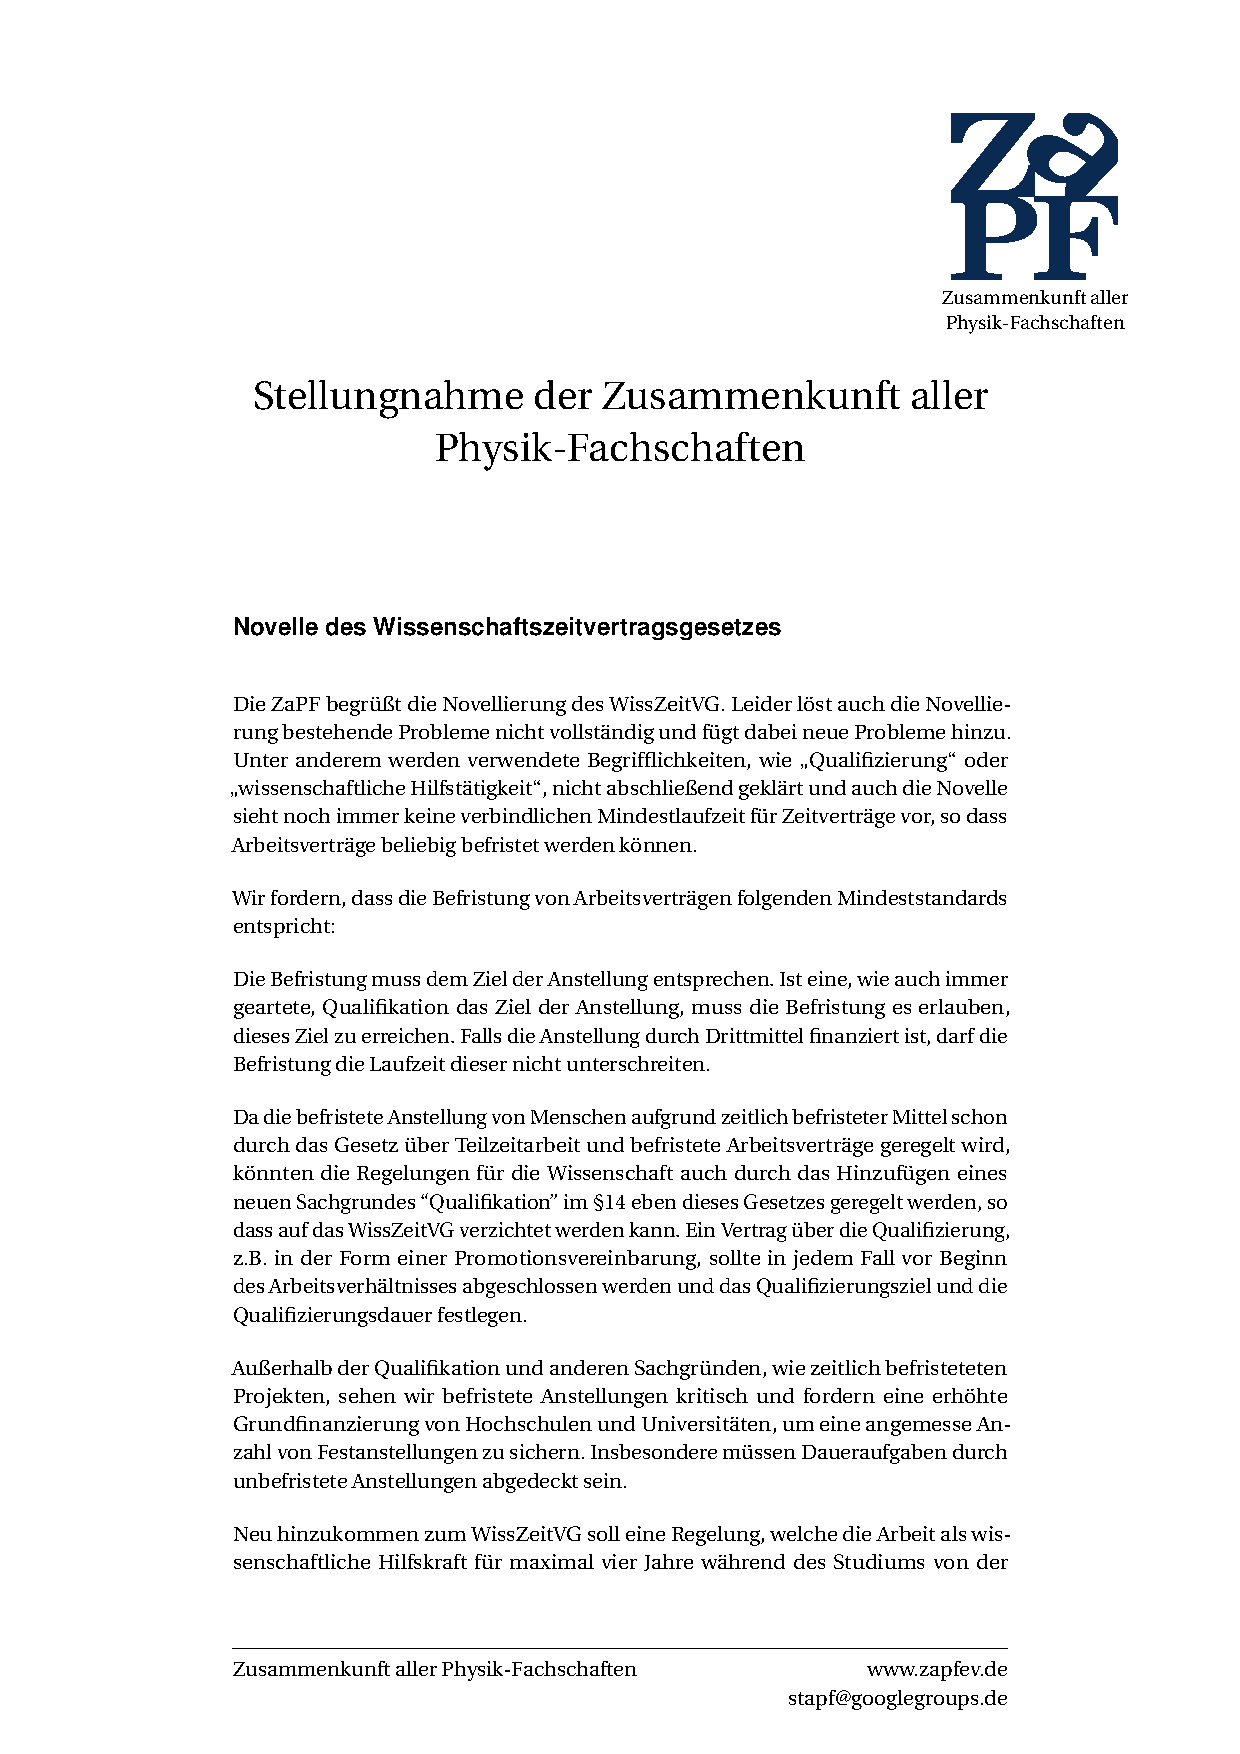
\includepdf[pages=-]{Stellungnahme_WiSe15_WissZeitVG.pdf}

\end{letter}
}

\massmail{Physikalische Gesellschaft e. V.\\Hauptstraße 5\\53604 Bad Honnef}{Sehr geehrte Damen und Herren,}
\massmail{Prof. Dr. Gert-Ludwig Ingold\\Institut für Physik\\Universität Augsburg\\86135 Augsburg}{Sehr geehrter Herr Prof. Dr. Ingold,}
\massmail{Hochschulrektorenkonferenz\\Generalsekretär: Dr. Jens-Peter Gaul\\Ahrstraße 39\\53175 Bonn}{Sehr geehrter Herr Dr. Gaul,}
\massmail{Sekretariat der Ständigen Konferenz der Kultusminister der Länder in der Bundesrepublik Deutschland\\Postfach 11 03 42\\10833 Berlin}{Sehr geehrte Damen und Herren,}
\massmail{Landesstudierendenvertretung\\c/o AStA-Geschäftsstelle\\Duale Hochschule Baden-Württemberg\\Friedrichstraße 14\\70174 Stuttgart}{Sehr geehrte Damen und Herren,}
\massmail{Zusammenschluss der bayerischen Studierendenvertretungen\\c/o Studierendenvertretung der LMU\\Leopoldstraße 15\\80802 München}{Sehr geehrte Damen und Herren,}
\massmail{LandesAstenKonferenz Berlin\\c/o AStA TU Berlin, Sekretariat TK 2\\Straße des 17. Juni 135\\10623 Berlin }{Sehr geehrte Damen und Herren,}
\massmail{SprecherInnenrat der BrandStuVe\\Am Neuen Palais 10\\14469 Potsdam}{Sehr geehrte Damen und Herren,}
\massmail{AStA der Goethe-Universität Frankfurt\\c/o LandesAstenKonferenz Hessen\\Mertonstr. 26-28\\60325 Frankfurt am Main}{Sehr geehrte Damen und Herren,}
\massmail{Landeskonferenz der Studierendenschaften Mecklenburg-Vorpommern\\Domstraße 12\\17489 Greifswald}{Sehr geehrte Damen und Herren,}
\massmail{LAT-NRW\\AStA an der Ruhr-Universität Bochum\\Studierendenhaus\\Universitätsstr. 150\\44780 Bochum}{Sehr geehrte Damen und Herren,}
\massmail{LandesAstenKonferenz Niedersachsen\\c/o AStA Uni Hannover\\Welfengarten 1\\30167 Hannover}{Sehr geehrte Damen und Herren,}
\massmail{LandesAStenKonferenz Rheinland-Pfalz\\c/o AStA der Uni Mainz\\Staudingerweg 21\\55128 Mainz}{Sehr geehrte Damen und Herren,}
\massmail{Konferenz Sächsischer Studierendenschaften\\c/o Student\_innenRat der Universität Leipzig\\Universitätsstraße 1\\04109 Leipzig}{Sehr geehrte Damen und Herren,}
\massmail{Otto-von-Guericke-Universität Magdeburg\\c/o Konferenz der Studierendenschaften Sachsen-Anhalts\\Postfach 4120\\39106 Magdeburg}{Sehr geehrte Damen und Herren,}
\massmail{AStA Uni Flensburg\\c/o LAK SH\\Auf dem Campus 1\\24943 Flensburg}{Sehr geehrte Damen und Herren,}
\massmail{Konferenz der Thüringer Studierendenschaften\\Carl-Zeiß-Straße 3\\07743 Jena}{Sehr geehrte Damen und Herren,}


%---------------------------------------------------------------------------
\end{document}
%---------------------------------------------------------------------------
